\documentclass[12pt]{article}

\usepackage{amsmath,enumitem,fullpage,soul,stoversymb}
\everymath{\displaystyle}
\allowdisplaybreaks
%\pagenumbering{gobble}

\usepackage{multicol}
\usepackage{tcolorbox}
\usepackage[margin=0.5in, top=1in, bottom=1in]{geometry}
\usepackage{tikz,tkz-euclide}
\usetkzobj{all}


\usepackage{amsthm}
\theoremstyle{definition}
\newtheorem{ex}{Example}

%\setenumerate{itemsep=0.25in}
\setlist[enumerate,1]{label=\arabic*., topsep=3mm, leftmargin=0.5in}
\setlist[itemize,1]{label=$\circ$, leftmargin=0.1875in, topsep=0mm}
\setlist[enumerate,2]{leftmargin=0.5in,itemsep=3mm}

\newcommand{\head}[2]{\noindent\textbf{#1}\\\indent{#2}\vspace{4mm}}
%\newcommand{\sol}{\noindent\textsc{Solution: }}
%\newcommand{\note}[1]{\hfill{\fbox{\text{{\footnotesize{#1}}}}}}
\newcommand{\sol}[1]{\begin{proof}[Soluion:]#1\end{proof}}
\newcommand{\opp}{\text{opposite}}
\newcommand{\adj}{\text{adjacent}}
\newcommand{\hyp}{\text{hypotenuse}}
\newcommand{\eqbox}[1]{\begin{tcolorbox}
	[colback=white,colframe=gray,boxrule=0.5pt,arc=0pt,top=3mm,bottom=3mm]#1\end{tcolorbox}\vspace{3mm}}

\begin{document}
	\noindent\begin{center}\Large{Trig Substitution}\end{center}
	\head{Introduction}{Trig substitution is a somewhat-confusing technique which, despite seeming arbitrary, esoteric, and complicated  (at best), is pretty useful for solving integrals for which no other technique we've learned thus far will work.}
	
	\head{Trig substitution list}{There are three main forms of trig substitution you should know:
	\begin{enumerate}[label=TS\arabic*.,leftmargin=0.75in]
		\item If you see $\sqrt{a^2-x^2}$: 
		\begin{itemize}
			\item Let $x=a\sin\theta$ for $-\pi/2\leq \theta\leq \pi/2$;
			\item then, $dx=a\cos\theta\,d\theta$;
			\item finally: 
		\end{itemize}
		$$\sqrt{a^2-x^2}=\sqrt{a^2-(a\sin\theta)^2}=\sqrt{a^2-a^2\sin^2\theta}=\sqrt{a^2(1-\sin^2\theta)}=\sqrt{a^2\cos^2\theta} = a\cos\theta$$

	
		\item If you see $\sqrt{a^2+x^2}$: 
		\begin{itemize}
			\item Let $x=a\tan\theta$ for $-\pi/2<\theta<\pi/2$;
			\item then, $dx=a\sec^2\theta\,d\theta$;
			\item finally:
		\end{itemize}
		$$\sqrt{a^2+x^2}=\sqrt{a^2+(a\tan\theta)^2}=\sqrt{a^2+a^2\tan^2\theta}=\sqrt{a^2(1+\tan^2\theta)}=\sqrt{a^2\sec^2\theta} = a\sec\theta$$
		
	
		\item If you see $\sqrt{x^2-a^2}$: 
		\begin{itemize}
			\item Let $x=a\sec\theta$ for $0\leq\theta<\pi/2$ (\textit{choose this if $x\geq a$}) \ul{or} $\pi\leq\theta<3\pi/2$ (\textit{choose this if $x\leq-a$});
			\item then, $dx=a\sec\theta\tan\theta\,d\theta$;
			\item finally:
		\end{itemize}
		$$\sqrt{x^2-a^2}=\sqrt{(a\sec\theta)^2-a^2}=\sqrt{a^2\sec^2\theta-a^2}=\sqrt{a^2(\sec^2\theta-1)}=\sqrt{a^2\tan^2\theta} = a\tan\theta$$
		
	\end{enumerate}}

	\head{Why trig substitution?}{Because integrals involving square roots are hard, and as the above table shows, using trig substitution can be a method for getting rid of square roots.}
	
	\head{Do I always need square roots?}{No. As we saw in class, you can use trig substitution even when you don't have square roots. In particular, if you have an integrand that looks like an expression \textbf{inside the square roots} shown in the above table, then you can use trig substitution. You should only do so if no other technique (e.g., $u$-substitution) works.
	
	Here are some examples.}
	
	\begin{ex} 
		Compute $$\int\frac{1}{\sqrt{x^2-9}}\,dx$$
	\end{ex}
	\sol{Here, no $u$-substitution will work, and so we use trig sub. From the above table, we have $\sqrt{x^2-9}=\sqrt{x^2-3^2}$, so letting $x=3\sec\theta$ and $dx=3\sec\theta\tan\theta\,d\theta$ transforms the square root into $\sqrt{9\sec^2\theta-9}=\sqrt{9\tan^2\theta}=3\tan\theta$. Hence, the integral becomes:
	$$\begin{array}{rcl}\int\frac{1}{\sqrt{x^2-9}}\,dx & = & \int\frac{1}{3\tan\theta}\left(3\sec\theta\tan\theta\,d\theta\right) \\[6mm] & = & \int\sec\theta\,d\theta\end{array}.$$
	This can be integrated directly using a clever trick, but should probably instead be considered an integral you should know.}

	\begin{ex} 
		Compute $$\int\frac{1}{(x^2-9)^2}\,dx$$
	\end{ex}
	\sol{This is almost identical to the first example. 
		
		Again, no $u$-substitution will work, and even though we have no square roots, we can use trig sub with $x=3\sec\theta$ and $dx=3\sec\theta\tan\theta\,d\theta$. Hence, the integral becomes:
		$$\begin{array}{rcl}\int\frac{1}{(x^2-9)^2}\,dx & = & \int\frac{1}{(9\tan^2\theta)^2}\left(3\sec\theta\tan\theta\,d\theta\right) \\[6mm] & = & \int\frac{\sec\theta}{27\tan^3\theta},d\theta\end{array}.$$
		At first glance, this probably appears no better, but rewriting $\tan$ and $\sec$ in terms of $\sin$ and $\cos$ tells us that 
		$$\int\frac{\sec\theta}{27\tan^3\theta},d\theta=\frac{1}{27}\int\csc\theta\cot^2\theta\,d\theta.$$
		This is considerably harder than the integral obtained in the first example but it's not undoable, and if you're clever with trig identities, you can get an answer here (which is more than you'd have gotten \textit{without} trig sub).}

	\begin{ex} 
		Compute $$\int\frac{x}{(x^2-9)^2}\,dx$$
	\end{ex}
	\sol{This is \textit{also} almost identical to the above examples, but there's one glaring difference: \textbf{You don't need trig substitution!}
		
	In particular, if we let $u=x^2+9$ and $du=2x\,dx$ (which implies that $x\,dx=du/2$), we can transform this integral into something elementary:
	
	$$\int\frac{x}{(x^2-9)^2}\,dx=\frac{1}{2}\int\frac{du}{u^2}.\qedhere$$}

	\head{Okay, so how do I solve a trig sub problem from \textit{beginning} to \textit{end}?}{As we've seen in class, it's not always straighforward.
		
	The good news is that we can break the problem into steps in a rather uniform way, regardless of what the problem looks like. First, we'll identify the process and then we'll look at an example.}
	
	\head{The process for finding integrals using trig substitution}{\vspace{-6mm}
		\begin{enumerate}[label=P\arabic*.]
			\item Try to fit your problem to one of the patterns $a^2-x^2$, $x^2+a^2$, or $x^2-a^2$.
			\begin{itemize}
				\item If you can't, you may have to do some \textit{preprocessing} of the problem. This can include:
				\begin{enumerate}
					\item completing the square;
					\item $u$-substitution;
					\item algebraic cleverness;
					\item some combination of the above.
				\end{enumerate}
			\end{itemize}
			\item Once you've done this, make the appropriate substitution of $x$ and $dx$. \textit{Make sure to use the simplifications (i.e., the ``square root removals'') that result from the trig substitution!}
			\item Simplify the integrand as needed and integrate.
			\begin{itemize}
				\item This may again require $u$-substitution, etc., and will oftentimes require knowledge of the trig integrals from the handout. \textit{Don't forget how to compute integrals in general!}
			\end{itemize}
			\item Reverse substitute until your result is in terms of $x$.
				\begin{itemize}
					\item If you used $u$-substitution along the way, you may also require additional back-substitutions.
					\item This will \textbf{definitely} require getting rid of the $\theta$ variables introduced by the trig substitution. To do this:
						\begin{enumerate}
							\item Draw a triangle to get rid of expressions involving $\sin\theta$, $\cos\theta$, $\tan\theta$, etc., which \textit{aren't} easily handled by the substitution itself.
							\vspace{6mm}
							\begin{center}
							\hspace{-1.25in}
								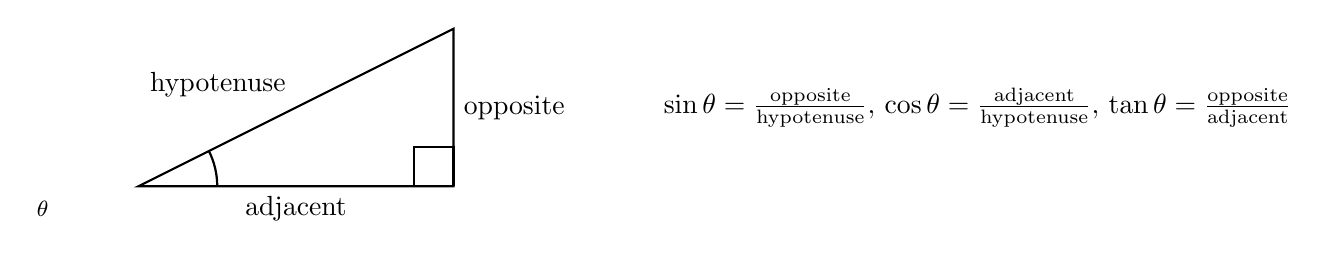
\begin{tikzpicture}[thick]
								\coordinate (O) at (0,0);
								\coordinate (A) at (-4,0);
								\coordinate (B) at (0,2);
								\draw (O)--(A)--(B)--cycle;
								
								\tkzLabelSegment[below=0pt](O,A){\adj}
								\tkzLabelSegment[right=0pt](O,B){\opp}
								\tkzLabelSegment[above left=0pt](A,B){\hyp}
								
								\tkzMarkRightAngle[fill=none,size=0.5,opacity=1](A,O,B)% square angle here
								
								\tkzMarkAngle[fill= none,size=1cm,%
								opacity=1](O,A,B)
								\tkzLabelAngle[pos = 1.25](B,A,O){\footnotesize{$\theta$}}
								
								\tkzLabelSegment[right=1in](O,B){$\sin{\theta}=\frac{\opp}{\hyp},\, \cos{\theta}=\frac{\adj}{\hyp},\, \tan{\theta}=\frac{\opp}{\adj}$}
								\end{tikzpicture}
							\end{center}
							\vspace{2mm}
							\textbf{Don't forget the Pythagorean Theorem:} $\adj^2+\opp^2=\hyp^2.$

							\item Use inverse trig functions to get rid of any $\theta$ that may exist \textit{outside} a trig function. \textbf{For example:} If you let $x=a\sin\theta$, then $\theta=\arcsin(x/a)$.
						\end{enumerate}
				\end{itemize}
		\end{enumerate}
	
	Let's look at an example.}

	\begin{ex}
		Find
		$$\int\frac{x^3}{\sqrt{x^2+100}}\,dx.$$
	\end{ex}
	\sol{Let's try to use the above outline to guide our methods.
		
	\begin{enumerate}[label=P\arabic*.,leftmargin=0.75in]
		\item Because the denominator is $\sqrt{x^2+100}=\sqrt{x^2+10^2}$, this integrand matches the substitution form TS2.
		
		\item As a result, we're going to use the following: Let $x=10\tan\theta$ for $-\pi/2 < \theta < \pi/2$ and $dx=10\sec^2\theta\,d\theta$. Simplifying inside the square root also yields:
		$$\sqrt{x^2+100}=\sqrt{(10\tan\theta)^2+100}=\sqrt{100(\tan^2\theta+1)}=10\sec\theta.$$
		Therefore, our integral now looks like:
		$$\int\frac{x^3}{\sqrt{x^2+100}}\,dx=\int\frac{(10\tan\theta)^3}{10\sec\theta}\left(10\sec^2\theta\,d\theta\right).$$
		
		\item Simplifying, we have
		$$\int\frac{(10\tan\theta)^3}{10\sec\theta}\left(10\sec^2\theta\,d\theta\right)=10^3\int\tan^3\theta\sec\theta\,d\theta.$$
		Recognizing the above integrand as a trig integral with odd power of $\tan$, we know (from the previous handout) that we can factor out a multiple of $\sec\theta\tan\theta$ with the intent of letting $u=\sec\theta$:
		$$\begin{array}{rcl}10^3\int\tan^3\theta\sec\theta\,d\theta & = & 1000\int(\sec\theta\tan\theta)\tan^2\theta\,d\theta \\ & = & 1000\int(\sec\theta\tan\theta)(\sec^2\theta-1)\,d\theta\end{array}$$
		Now, we use $u$-substitution with $u=\sec\theta$, $du=\sec\theta\tan\theta\,d\theta$:
		$$\begin{array}{rcl}1000\int(\sec\theta\tan\theta)(\sec^2\theta-1)\,d\theta & = & 1000\int(u^2-1)\,du \\ & = & 1000\left(\frac{1}{3}u^3+u\right)+C.\end{array}$$
		
		\item The integral found above is in terms of $u$ while the the original question was in terms of $x$. This means we need to back-substitute.
		
		The first substitution is easy: Because $u=\sec\theta$,
		\begin{equation}
		\label{ThetaInt1}
		1000\left(\frac{1}{3}u^3+u\right)+C=1000\left(\frac{1}{3}\sec^3\theta+\sec\theta\right)+C.\end{equation}
		Now, we have a result in terms of $\theta$: This means we have to do the trig reversal (i.e., the \textit{trickier} back-substitution).
		
		\textbf{What we know:} $x=10\tan\theta$ (because that's what we substituted). This implies that $\tan\theta=x/10$ (and that $\theta=\arctan(x/10)$, if we need it), and using what we know about $\tan$,
		$$\frac{x}{10}=\tan\theta=\frac{\opp}{\adj}.$$
		
		\textbf{What we do next:} Draw a right triangle, label a non-right angle $\theta$, and fill in the sides with what you know.
		
		\begin{center}
		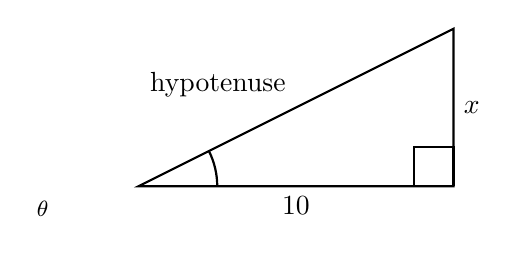
\begin{tikzpicture}[thick]
		\coordinate (O) at (0,0);
		\coordinate (A) at (-4,0);
		\coordinate (B) at (0,2);
		\draw (O)--(A)--(B)--cycle;
		
		\tkzLabelSegment[below=0pt](O,A){$10$}
		\tkzLabelSegment[right=0pt](O,B){$x$}
		\tkzLabelSegment[above left=0pt](A,B){\hyp}
		
		\tkzMarkRightAngle[fill=none,size=0.5,opacity=1](A,O,B)% square angle here

		\tkzMarkAngle[fill= none,size=1cm,%
		opacity=1](O,A,B)
		\tkzLabelAngle[pos = 1.25](B,A,O){\footnotesize{$\theta$}}
		\end{tikzpicture}
		\end{center}
	
		Next, solve for the remaining side using the Pythagorean theorem:
		$$10^2+x^2=\hyp^2\implies\hyp^2=x^2+100.$$
		Taking square roots allows you to fill in the updated triangle:
		
		\begin{center}
			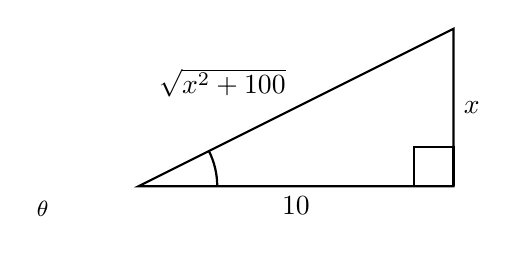
\begin{tikzpicture}[thick]
			\coordinate (O) at (0,0);
			\coordinate (A) at (-4,0);
			\coordinate (B) at (0,2);
			\draw (O)--(A)--(B)--cycle;
			
			\tkzLabelSegment[below=0pt](O,A){$10$}
			\tkzLabelSegment[right=0pt](O,B){$x$}
			\tkzLabelSegment[above left=0pt](A,B){$\sqrt{x^2+100}$}
			
			\tkzMarkRightAngle[fill=none,size=0.5,opacity=1](A,O,B)% square angle here
			
			\tkzMarkAngle[fill= none,size=1cm,%
			opacity=1](O,A,B)
			\tkzLabelAngle[pos = 1.25](B,A,O){\footnotesize{$\theta$}}
			\end{tikzpicture}
		\end{center}
	
		Now, from \eqref{ThetaInt1}, we know we need an expression for $\sec\theta$. But
		$$\sec\theta=\frac{\hyp}{\adj}=\frac{\sqrt{x^2+100}}{10},$$
		and so \eqref{ThetaInt1} becomes
		$$1000\left(\frac{1}{3}\sec^3\theta+\sec\theta\right)+C=1000\left(\frac{1}{3}\left(\frac{\sqrt{x^2+100}}{10}\right)^3+\frac{\sqrt{x^2+100}}{10}\right)+C.$$
		
		After all that, what we have is what we want:
	\end{enumerate}

	\eqbox{$$\int\frac{x^3}{\sqrt{x^2+100}}\,dx=1000\left(\frac{1}{3}\left(\frac{\sqrt{x^2+100}}{10}\right)^3+\frac{\sqrt{x^2+100}}{10}\right)+C.\qedhere$$}}

	\head{But, we can still use trig substitution on things that don't look like the three cases in the trig table! I DON'T NEED PERFECT SQUARES!}{Indeed you don't, and the reason is because you can complete the square on an arbitrary quadratic polynomial $ax^2+bx+c$ to get something which looks like
		$$ax^2+bx+c=a\left(x+\frac{b}{2a}\right)^2+\frac{4c-b}{4a},$$
	upon which you can \textit{then} do $u$-substitution with $u=x+b/(2a)\implies du=dx.$}

	\head{Uh...\textit{hwhat?!}}{Let's look at the example we did in class yesterday.}
	
	\begin{ex}
		Evaluate $$\int\frac{dx}{(x^2-6x+11)^2}.$$
	\end{ex}
	\sol{First, we note that we don't have a square root, though as we've seen, that's not a problem.
		
	We again use the outline to guide our methods.
	
	\begin{enumerate}[label=P\arabic*.,leftmargin=0.75in]
		\item This doesn't match any of TS1, TS2, or TS3, and so we have to do \textit{preprocessing}. 
		
		Now: We don't have a sum or difference of perfect squares which hints that we want to \textbf{complete the square} on the denominator expression $x^2-6x+11$, and to do that, we want to fill in $\square$ so that we have the following:
		$$x^2-6x+11=\underbrace{x^2-6x+\square}_{\text{should be a perfect square!}}+11-\square.$$
		Said differently: we want to find a number $\square$ that we can add and subtract to make $x^2-6x+\square$ a perfect square. 
		
		To do this, we let $\square=\left(\frac{-6}{2}\right)^2=9$, because $x^2-6x+9=(x-3)^2$. Thus, we rewrite: $x^2-6x+11=(x-3)^2+2$, and hence
		$$\int\frac{dx}{(x^2-6x+11)^2}=\int\frac{dx}{\left((x-3)^2+2\right)^2}.$$
		
		Notice that we're \textit{almost} matching TS2, except that the ``perfect square variable'' isn't a single variable but is instead $x-3$. To rectify, let $u=x-3$, $du=dx$, and rewrite:
		
		$$\int\frac{dx}{\left((x-3)^2+2\right)^2}=\int\frac{du}{\left(u^2+2\right)^2}.$$
		
		At this point, the denominator is a TS2 form $u^2+2=u^2+(\sqrt{2})^2$ (i.e., $a=\sqrt{2}$).
		
		\item It's time to make the trig sub indicated in TS2, so we let $u=\sqrt{2}\tan\theta$ for $-\pi/2<\theta<\pi/2$ so that $du=\sqrt{2}\sec^2\theta\,d\theta$:
		$$\int\frac{du}{\left(u^2+2\right)^2} = \int\frac{\sqrt{2}\sec^2\theta\,d\theta}{\left((\sqrt{2}\tan\theta)^2+2\right)^2}.$$
		
		\item Now, we simplify and integrate:
		\begin{align*}\int\frac{du}{\left(u^2+2\right)^2} & = \int\frac{\sqrt{2}\sec^2\theta\,d\theta}{\left((\sqrt{2}\tan\theta)^2+2\right)^2} \\ & =  \int\frac{\sqrt{2}\sec^2\theta\,d\theta}{\left(2\tan^2\theta+2\right)^2}\\ & =  \int\frac{\sqrt{2}\sec^2\theta\,d\theta}{\left(2(\tan^2\theta+1)\right)^2}\\ & = \frac{\sqrt{2}}{4}\int\frac{\sec^2\theta\,d\theta}{(\tan^2\theta+1)^2}\\ & =  \frac{\sqrt{2}}{4}\int\frac{\sec^2\theta\,d\theta}{(\sec^2\theta)^2}\\ & =  \frac{\sqrt{2}}{4}\int\frac{d\theta}{\sec^2\theta}=\frac{\sqrt{2}}{4}\int\cos^2\theta\,d\theta.\end{align*}
		
		Recognizing the integrand as an even power of cosine, we refer to our handout on trig integrals and find the identity $\cos^2x=(1+\cos(2x))/2$. Therefore:
		$$\begin{array}{rcl}\frac{\sqrt{2}}{4}\int\cos^2\theta\,d\theta & = & \frac{\sqrt{2}}{4}\int\frac{1+\cos(2\theta)}{2}\,d\theta\\[6mm] & = & \frac{\sqrt{2}}{8}\int\left(1+\cos(2\theta)\right)\,d\theta\\[6mm] & = & \frac{\sqrt{2}}{8}\left(\theta+\frac{1}{2}\sin(2\theta)\right)+C.\end{array}.$$
		Note that the integral of $\cos(2\theta)$ with respect to $\theta$ requires $u$-substitution with $u=2\theta$.
		
		Also, because the triangle we draw in P4 requires things to be in terms of $\theta$ rather than $2\theta$, we do some algebra and trig (noting that $\sin(2\theta)=2\sin\theta\cos\theta$ from the list of identities):
		\begin{align}[rcl]\frac{\sqrt{2}}{8}\left(\theta+\frac{1}{2}\sin(2\theta)\right)+C & = \frac{\sqrt{2}}{8}\left(\theta+\frac{1}{2}(2\sin\theta\cos\theta)\right)+C\nonumber\\ & = \label{ThetaInt2} \frac{\sqrt{2}}{8}\left(\theta+\sin\theta\cos\theta\right)+C.\end{align}
		
		\item Now, we use $u=\sqrt{2}\tan\theta$ to deduce that $u/\sqrt{2}=\tan\theta$, that $\theta=\arctan(u/\sqrt{2})$, and to label our triangle:
		
		\begin{center}
			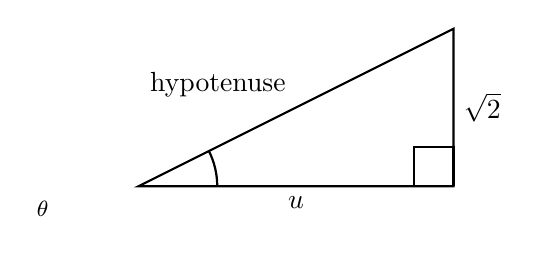
\begin{tikzpicture}[thick]
			\coordinate (O) at (0,0);
			\coordinate (A) at (-4,0);
			\coordinate (B) at (0,2);
			\draw (O)--(A)--(B)--cycle;
			
			\tkzLabelSegment[below=0pt](O,A){$u$}
			\tkzLabelSegment[right=0pt](O,B){$\sqrt{2}$}
			\tkzLabelSegment[above left=0pt](A,B){\hyp}
			
			\tkzMarkRightAngle[fill=none,size=0.5,opacity=1](A,O,B)% square angle here
			
			\tkzMarkAngle[fill= none,size=1cm,%
			opacity=1](O,A,B)
			\tkzLabelAngle[pos = 1.25](B,A,O){\footnotesize{$\theta$}}
			\end{tikzpicture}
		\end{center}
	
		Using the Pythagorean theorem, we get that
		$$\hyp=\sqrt{u^2+(\sqrt{2})^2}=\sqrt{u^2+2},$$
		so the completed triangle is as follows:
	
		\begin{center}
			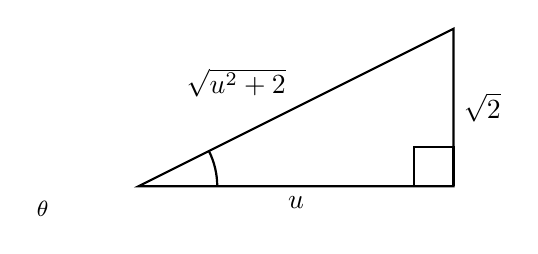
\begin{tikzpicture}[thick]
			\coordinate (O) at (0,0);
			\coordinate (A) at (-4,0);
			\coordinate (B) at (0,2);
			\draw (O)--(A)--(B)--cycle;
			
			\tkzLabelSegment[below=0pt](O,A){$u$}
			\tkzLabelSegment[right=0pt](O,B){$\sqrt{2}$}
			\tkzLabelSegment[above left=0pt](A,B){$\sqrt{u^2+2}$}
			
			\tkzMarkRightAngle[fill=none,size=0.5,opacity=1](A,O,B)% square angle here
			
			\tkzMarkAngle[fill= none,size=1cm,%
			opacity=1](O,A,B)
			\tkzLabelAngle[pos = 1.25](B,A,O){\footnotesize{$\theta$}}
			\end{tikzpicture}
		\end{center}
	
		Now we know that $\theta=\arctan(u/\sqrt{2})$, $\sin\theta=\sqrt{2}/\sqrt{u^2+2}$, and $\cos\theta=u/\sqrt{u^2+2}$. Therefore, the integral in \eqref{ThetaInt2} becomes
		$$\frac{\sqrt{2}}{8}\left(\theta+\sin\theta\cos\theta\right)+C=\frac{\sqrt{2}}{8}\left(\arctan\left(\frac{u}{\sqrt{2}}\right)+\left(\frac{\sqrt{2}}{\sqrt{u^2+2}}\right)\left(\frac{u}{\sqrt{u^2+2}}\right)\right)+C,$$
		and because the original substitution had the form $u=x-3$, we're done:
	\end{enumerate}

	\eqbox{$$\int\frac{dx}{(x^2-6x+11)^2}=\frac{\sqrt{2}}{8}\left(\arctan\left(\frac{x-3}{\sqrt{2}}\right)+\left(\frac{\sqrt{2}}{\sqrt{(x-3)^2+2}}\right)\left(\frac{x-3}{\sqrt{(x-3)^2+2}}\right)\right)+C.\qedhere$$}}

	And, because that last example was long and difficult, there's one more you should consider:
	
	\begin{ex}
		Evaluate $$\int\frac{x}{\sqrt{3-2x-x^2}}\,dx.$$
	\end{ex}
	\sol{This solution can be found on pages 482---483 of the textbook.
	
	Before referring to that solution, try to do the problem on your own \textit{first} using P1---P4 to guide you.}
\end{document}